%-------------------------------
%	DOCUMENT SETTINGS
%-------------------------------
\documentclass[a4paper]{article}

\setlength{\hoffset}{-3.2cm}
\setlength{\voffset}{-3cm}
\setlength{\textwidth}{18.7cm}
\setlength{\textheight}{25.5cm}
\setlength{\parskip}{0pt}
\setlength{\parindent}{0in}

%----------------------------------------------------------------------------------------
%	PACKAGES AND OTHER DOCUMENT CONFIGURATIONS
%----------------------------------------------------------------------------------------

\usepackage{minted}
\usepackage{mathtools}
\usepackage[utf8]{inputenc} % Use UTF-8 encoding
\usepackage{microtype} % Slightly tweak font spacing for aesthetics
\usepackage[english]{babel} % Language hyphenation and typographical rules
\usepackage{amsthm, amsmath, amssymb} % Mathematical typesetting
\usepackage{float} % Improved interface for floating objects
\usepackage[final, colorlinks = true, linkcolor = black, citecolor = black]{hyperref} % For hyperlinks in the PDF
\usepackage{dsfont}
\DeclarePairedDelimiter\abs{\lvert}{\rvert}%
\usepackage{cancel}
\usepackage{charter} % Use the Charter font
\usepackage{graphicx, multicol} % Enhanced support for graphics
\usepackage{xcolor} % Driver-independent color extensions
\usepackage{booktabs} % Enhances quality of tables
\usepackage{tikz-qtree} % Easy tree drawing tool
% Configuration for b-trees and b+-trees, !uses style file!
%\usepackage[backend=biber,style=numeric,
%            sorting=nyt]{biblatex} % Complete reimplementation of bibliographic facilities
%\addbibresource{ecl.bib}
\usepackage[yyyymmdd]{datetime} % Uses YEAR-MONTH-DAY format for dates
\renewcommand{\dateseparator}{-} % Sets dateseparator to '-'
\usepackage{fancyhdr} % Headers and footers
\pagestyle{fancy} % All pages have headers and footers
\fancyhead{}\renewcommand{\headrulewidth}{0pt} % Blank out the default header
\fancyfoot[L]{} % Custom footer text
\fancyfoot[C]{} % Custom footer text
\fancyfoot[R]{\thepage} % Custom footer text
\newcommand{\note}[1]{\marginpar{\scriptsize \textcolor{red}{#1}}} % Enables comments in red on margin

%----------------------------------------------------------------------------------------
%	CUSTOM COMMANDS
%----------------------------------------------------------------------------------------

\newcommand{\R}{\mathbb{R}}
\newcommand{\E}{\mathbb{E}}
\newcommand{\I}{\mathbb{I}}
\newcommand{\Var}{\text{Var}}
% Para poner sonrisa sobre puntos suspensivos. Uso: \overplace{n}{\dotsc}
\newcommand{\overplace}[2]{%
	\overset{\substack{#1\\\smile}}{#2}%
}

\begin{document}
	
%-------------------------------
%	TITLE SECTION
%-------------------------------

\fancyhead[C]{}
\hrule \medskip % Upper rule
\begin{minipage}{0.295\textwidth} 
	\raggedright
	\footnotesize
	José Antonio Álvarez Ocete \hfill\\   
	77553417Q \hfill\\
	joseantonio.alvarezo@estudiante.uam.es
\end{minipage}
\begin{minipage}{0.4\textwidth} 
	\centering 
	\large 
	Final \\ 
	\normalsize 
	Procesos estocásticos discretos\\ 
\end{minipage}
\begin{minipage}{0.295\textwidth} 
	\raggedleft
	\today\hfill\\
\end{minipage}
\medskip\hrule 
\bigskip

%-------------------------------
%	CONTENTS
%-------------------------------

\section*{Ejercicio I.}

\textbf{Enunciado.} En los apuntes hay el ejemplo del \emph{gambler's ruin} como cadena de Markov:

\begin{figure}[H]
	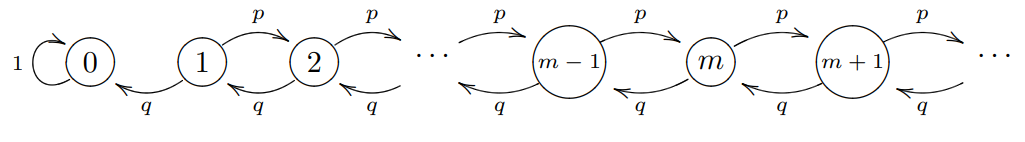
\includegraphics[scale=.6]{figures/gamblers_ruin}
	\centering
\end{figure}

Donde estar en el nodo $i$ implica tener $i$ Euros, y $p$ y $q=1-p$ son las probabilidades de ganar y perder respectivamente en cada repetición del juego. \\

\textbf{Apartado a)} Hacer un gráfico del número medio de jugadas que el jugador puede hacer antes de arruinarse en función del dinero inicial. En cada jugada se juega $1$ Euro, y el juego es ecuo (el jugador tiene una probabilidad $p=1/2$ de ganar). \\

Sabemos por el estudio teórico realizado para este problema que en el caso de $p=q=\frac{1}{2}$, el jugador convergerá a arruinarse tarde o temprano. Sin embargo, la simulación puede tomar un tiempo arbitrariamente alto de tiempo si el dinero inicial es alto. Es por ello que hemos de poner un límite al número de iteraciones máximo que ejecutaremos nuestra simulación. Consideramos que $10^5$ es una cantidad aceptable de iteraciones para los bajos valores de dinero inicial que utilizaremos. Si se alcanza ese número de iteraciones podemos considerar que el jugador "se arruina en tiempo $10^5$, que es básicamente infinito. \\

Implementamos la simulación de esta cadena de Markov y la ejecutamos $20$ veces, computando su media. Realizar esta simulación en múltiples ocasiones y utilizar la media es imprescindible para obtener resultados representativos en procesos de Monte Carlo como este. Cabe destacar que para cualquiera de estos experimentos fijamos la semilla a $123$ para poder reproducirlos posteriormente.
	
\begin{minted}{python}
def simulate_gambler_step(p=1/2):
	""" 
		Simulates a single step of the gambler's ruin
		- p: the probability of winning
		- returns: 1 if won, -1 if lost
	"""
	r = random.uniform(0, 1)
	return 1 if r <= p else -1

def simulate_gamblers_ruin(initial_money, p=1/2, max_steps=10**6):
	"""
		Simulates a gambler's ruin markov chain.
		- initial_money: the starting node
		- p: the probability of winning at each step
		- max_steps: the max number of steps to be comptued
		- returns: time taken to ruin the gambler. If max_steps is reached
		without ruining the gambler, return max_steps instead.
	"""
	money = initial_money
	steps = 0
	while money > 0 and steps <= max_steps:
	steps += 1
	money += simulate_gambler_step(p)
	return steps

def plot_mean_ruin_time(max_initial_money=50, n=20, max_steps=10**5, p=1/2):
	"""
		Plots the mean time for a gambler's to ruin themself, against the initial money.
		- max_initial_money: max initial money to be plotted
		- n: the number of executions per initial money value
		- max_steps: the max number of steps to be comptued
		- p: the probability of winning at each step
	"""
	# Compute times
	initial_money_range = np.arange(1, max_initial_money)
	mean_times = [
		np.mean( [simulate_gamblers_ruin(initial_money, p=p, max_steps=max_steps)
				for _ in range(n)] )
		for initial_money in initial_money_range
	]

	# Plotting
	plt.figure(figsize=(12,6))
	plt.plot(initial_money_range, mean_times, '-o')
	plt.legend(['Mean time to ruin', 'Max iterations'])
	plt.xlabel('Initial money')
	plt.ylabel('Mean time to ruin in {} iterations'.format(n))
	plt.title('Gambler\' ruin simulation')
	plt.show()
	
random.seed(123)
plot_mean_ruin_time(max_steps=10**5)
\end{minted}
	
\begin{figure}[H]
	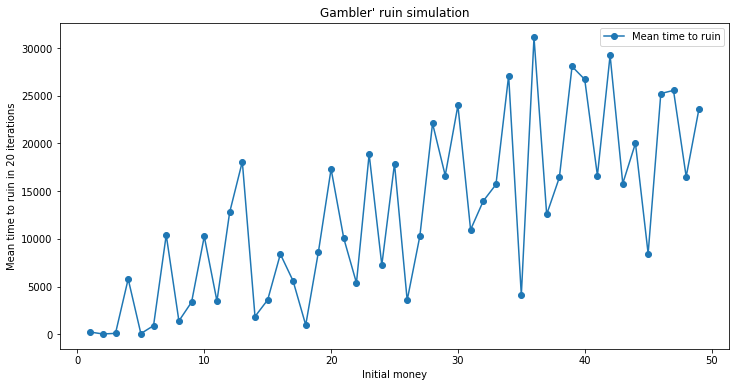
\includegraphics[scale=.6]{figures/gambler1}
	\centering
	\caption{Mean time of 50 simulations of Gambler's Ruin process}
\end{figure}

\textbf{Apartado b)} Estimar media y varianza (usar unas 20 ejecuciones, deberían ser más que suficientes) considerando un dinero inicial de $\{1, \ldots, 50\}$ euros. Indicar media y varianza. ¿Cómo varían la media y la varianza cuando aumenta el dinero inicial? \\

Para este segundo apartado repetimos el experimento anterior calculando también la desviación típica sobre esas 20 repeticiones. Puesto que queremos visualizar cómo afecta la varianza de las ejecuciones a la salida del modelo, representaremos en el gráfica también la desviación típica. Adicionalmente, como estimación más realista de la dispersión de las medidas podemos utilizar un intervalo de confianza. En particular, hemos utilizado intervalos de confianza que asumen que las mediciones se distribuyen según una distribución normal, lo que no tendría por qué ser exactamente cierto. La fórmula utilizada para dichos intervalos es la siguiente:

\[
	\text{IC} = [ \bar x - \frac{\sigma \cdot z}{\sqrt n}, \bar x + \frac{\sigma \cdot z}{\sqrt n}  ]
\]

Donde para nivel de significación $\alpha = 0.05$, $z_{1 - 0.05/2} = z_{0.975}$ es el percentil $0.975$ de la distribución normal. Veámos los resultados obtenidos:

\begin{minted}{python}
def mean_and_std_of_ruin_time(initial_money, n=20, max_steps=10**5, p=1/2):
	times = [simulate_gamblers_ruin(initial_money, p=p, max_steps=max_steps)
	for _ in range(n) ]
	return np.mean(times), np.std(times)

def compute_clipped_CI(mean, std, n, alpha=0.05):
	z = stats.norm.ppf(1 - alpha/2)
	std_error = abs(std * z / np.sqrt(n))
	return max(mean - std_error, 0), mean + std_error

def plot_ruin_time_estimation(max_initial_money=50, n=20, max_steps=10**5, p=1/2):
	"""
		Plots the mean time for a gambler's to ruin themself, against the initial money.
		- max_initial_money: max initial money to be plotted
		- n: the number of 
		- p: the probability of winning at each step
	"""
	# Compute times
	initial_money_range = np.arange(1, max_initial_money)
	mean_and_stds = np.array([mean_and_std_of_ruin_time(initial_money, n=n, max_steps=max_steps, p=p)
								for initial_money in initial_money_range])
	intervals = np.array([ compute_clipped_CI(mean, std, n) for mean, std in mean_and_stds])
	CI_std_min, CI_std_max = np.max(mean_and_stds[:,0] - mean_and_stds[:,1], 0), mean_and_stds[:,0] + mean_and_stds[:,1]
	
	# Plotting
	plt.figure(figsize=(12,6))
	plt.plot(initial_money_range, mean_and_stds[:,0], '-o')
	plt.fill_between(initial_money_range, CI_std_min, CI_std_max, color='green', alpha=.3)
	plt.fill_between(initial_money_range, intervals[:,0], intervals[:,1], color='b', alpha=.3)
	plt.legend(['Mean time to ruin', '+- Std', 'Confidence interval'])
	plt.xlabel('Initial money')
	plt.ylabel('Mean time to ruin in {} iterations'.format(n))
	plt.title('Gambler\' ruin simulation')
	plt.show()
	
random.seed(123)
plot_ruin_time_estimation()
\end{minted}

\begin{figure}[H]
	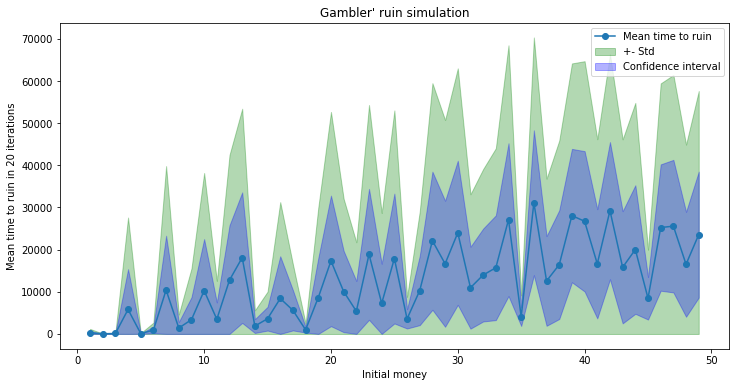
\includegraphics[scale=.6]{figures/gambler2}
	\centering
	\caption{Mean, std and normal confidence interval for the ruining time, 20 executions.}
\end{figure}

Vemos en la figura anterior como tanto el intervalo de confianza como la deviación típica aumentan gradualmente al incrementar el dinero inicial. Algunas de estas simulaciones acababan llegando al límite de $10^5$ impuesto. \\

Vemos también como hay mucha fluctuación para los valores medios. Por ejemplo, apreciamos cierto punto entre $30$ y $40$ euros iniciales que toma valores bajísimos en todas sus ejecuciones (por esto la desviación típica es también tan pequeña). Esto nos indica que quizás $20$ ejecuciones para esta simulación no nos dan una estimación correcta de la media y varianza. Volvemos a lanzar el experimento para $100$ ejecuciones y obtenemos los siguientes resultados:

\begin{minted}{python}
random.seed(123)
plot_ruin_time_estimation(n=100)
\end{minted}

\begin{figure}[H]
	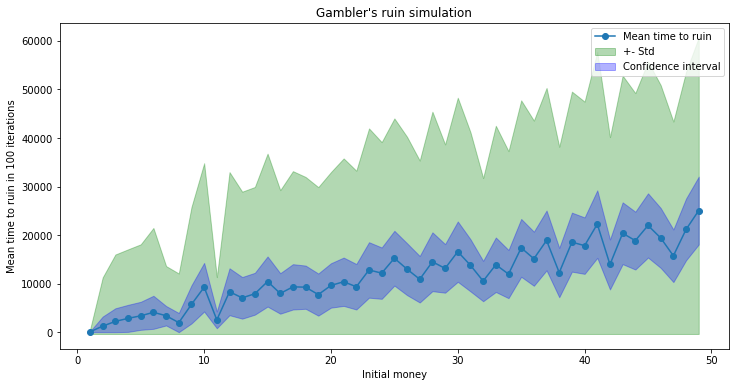
\includegraphics[scale=.6]{figures/gambler2_1}
	\centering
	\caption{Mean, std and normal confidence interval for the ruining time, 100 executions.}
\end{figure}

Podemos apreciar que se reduce enormemente la comentada variabilidad: los valores obtenidos están mucho más alineados no hay tanta oscilación. Sin embargo, han aumentado tremendamente los valores medios entre este experimento y el anterior. Este se debe a que muchas más simulaciones han alcanzado el límite de tiempo impuesto, y la media sube enormemente. A pesar de ello, \textbf{podemos deducir que tanto el número de simulaciones que alcanzan el límite como el tiempo medio crecen de forma lineal}. Este resultado será clave para el próximo apartado. \\

Por otro lado, es claro que al imponer este límite en las iteraciones estamos introduciendo un sesgo en los resultados: el tiempo medio aumenta considerablemente. Sin embargo, imponer un límite más alto sólo introduce un mayor sesgo. La conclusión es clara: \textbf{es realmente complicado obtener estimaciones insesgadas y precisas del tiempo que tarda el jugador en arruinarse}, debido al elevadísimo tiempo que medio que conlleva. \\

\textbf{Apartado c)} Dar una estimación de la función $T(e)$ que da el tiempo medio necesario para arruinarse en función de la cantidad inicial de dinero, e. Según esta función, ¿cuánto tarda el jugador en arruinarse si empieza a jugar con 200 Euros? \\

Por el resultado expuesto en el apartado anterior, sabemos que una estimación lineal será adecuada. Es por ello que utilizaremos regresión lineal. Sin embargo, como también ha sido previamente comentado, cuantas más ejecuciones realizamos mayor será el sesgo introducido. Por otro lado, para pocas iteraciones, la varianza es muy alta y tendremos un mayor error. Realizaremos pues dos estimaciones: para $20$ y $100$ ejecuciones respetivamente.

\begin{minted}{python}
def plot_ruin_time_regression(max_initial_money=50, n=20, max_steps=10**5, p=1/2, display_prediction=True):
	"""
	Plots the mean time for a gambler's to ruin themself, against the initial money.
	- max_initial_money: max initial money to be plotted
	- n: the number of 
	- p: the probability of winning at each step
	"""
	# Compute times
	initial_money_range = np.arange(1, max_initial_money)
	mean_and_stds = np.array([mean_and_std_of_ruin_time(initial_money, n=n, max_steps=max_steps, p=p)
								for initial_money in initial_money_range])
	intervals = np.array([ compute_clipped_CI(mean, std, n) for mean, std in mean_and_stds])
	CI_std_min, CI_std_max = np.max(mean_and_stds[:,0] - mean_and_stds[:,1], 0), mean_and_stds[:,0] + mean_and_stds[:,1]

	# Compute regression
	X = initial_money_range.reshape(-1, 1)
	y = mean_and_stds[:,0].reshape(-1, 1)
	reg_model = LinearRegression().fit(X, y)
	predictions = reg_model.predict(X)
	
	# Display the prediction for 200 initial money
	if display_prediction:
		result = reg_model.predict(np.array([[200]]))
		print('Prediction for 200 initial money (n={}): {}'.format(n, result[0,0]))

	# Plotting
	plt.figure(figsize=(12,6))
	plt.plot(initial_money_range, mean_and_stds[:,0], '-o')
	plt.plot(initial_money_range, predictions, color='r')
	plt.fill_between(initial_money_range, CI_std_min, CI_std_max, color='green', alpha=.3)
	plt.fill_between(initial_money_range, intervals[:,0], intervals[:,1], color='b', alpha=.3)
	plt.legend(['Mean time to ruin', 'linear regression', '+- Std', 'Confidence interval'])
	plt.xlabel('Initial money')
	plt.ylabel('Mean time to ruin in {} iterations'.format(n))
	plt.title('Gambler\'s ruin simulation')
	plt.show()
	
random.seed(123)
plot_ruin_time_regression()
\end{minted}

\begin{minted}{bash}
	Prediction for 200 initial money (n=20): 94067.22283163268
\end{minted}

\begin{figure}[H]
	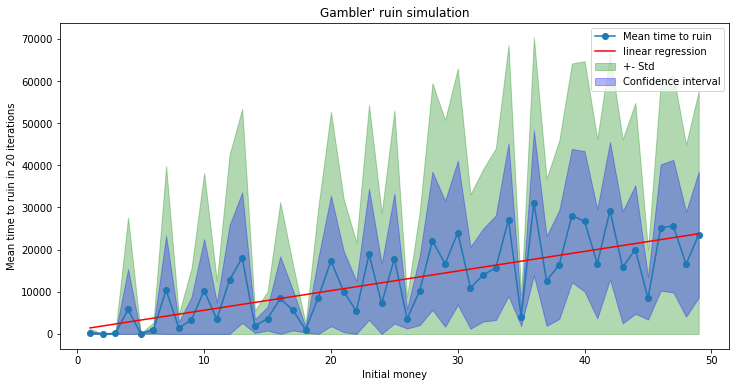
\includegraphics[scale=.6]{figures/gambler3}
	\centering
	\caption{Lineal regression for the ruining time, 100 executions.}
\end{figure}


\begin{minted}{python}
random.seed(123)
plot_ruin_time_regression(n=100)
\end{minted}

\begin{minted}{bash}
	Prediction for 200 initial money (n=100): 83077.38566326529
\end{minted}

\begin{figure}[H]
	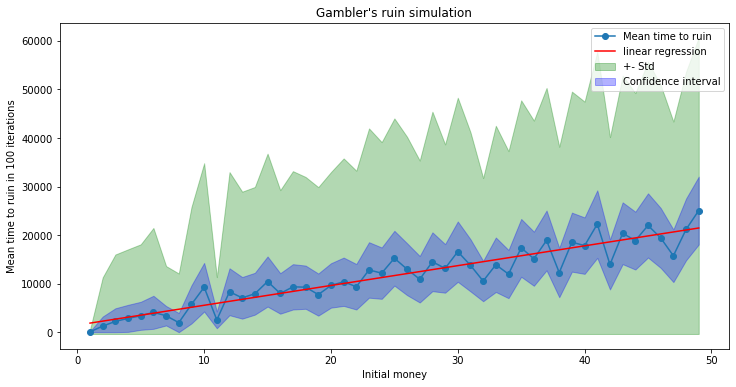
\includegraphics[scale=.6]{figures/gambler3_1}
	\centering
	\caption{Lineal regression for the ruining time, 100 executions.}
\end{figure}

Obtenemos así dos predicciones, entre las cuales la más cercana al valor real -sesgado por el límite introducido- será la segunda: $83077.39$ será el tiempo medio que el jugador tardará en arruinarse. Suponiendo que una iteración del juego tarde $1$ minuto, el jugador tardaría en arruinarse, de media, $57.69$ días (sin parar de jugar).

\section*{Ejercicio III.}

\textbf{Apartado a)} Crear cuatro sistemas dinámicos del tipo:

\[
	x_{t+1} = A x_t + B u_t + w_t
	z_t = C x_t + v_t
\]

con $x_t \in \R^4, u_t \in \R, z_t \R^2$, y

\[
	B = \begin{pmatrix} 1 & 1 & 1 & 1 \end{pmatrix}'
	C = \begin{pmatrix}
		1 & 0 & 0 & 0 \\
		0 & 1 & 0 & 0
	\end{pmatrix}'
\]

Los sistema se distinguen por la matrix $A$, que es, por cada sistema una de las cuatro matrices generadas usando la función \emph{mk\_mat} (en el fichero \emph{kalman\_aux}) a partir de las siguientes listas de autovalores:

\[
	\Lambda_1 = \begin{pmatrix} 0.2 & 0.2 & 0 & -0.1 \end{pmatrix}
	\Lambda_2 = \begin{pmatrix} 0.99 & 0.1 & 0 & -0.1 \end{pmatrix}
	\Lambda_3 = \begin{pmatrix} 1 & 0.1 & 0 & -0.1 \end{pmatrix}
	\Lambda_4 = \begin{pmatrix} 0.2 & 0.1 & 0 & -1 \end{pmatrix}
\]

Los ruidos $w_t \in \R^4$ y $v_t \in \R^2$ son gausiano y tienen matrices de covarianza

\[
	Q = \sigma_w \I_4
	R = \sigma_v \I_2
\]

\textbf{Solución:} Creamos una clase que define este sistema dinámico. Para ello hemos de tener en cuenta que la matriz $A$ es variable y será pasado como parámetro al constructor. El resto de parámetros del sistema tendrán valores por defecto para no tener que preocuparnos por ellos sin perder generalidad. \\

Para los valores iniciales tomaremos $x_0 = \hat x_0 = 0$, luego $P_0 = 0$. Esto no será especialmente relevante: las primeras iteraciones no podremos predecir bien ya que no conocemos los estados anteriores. Tras esto, el sistema se estabilizará y los errores que aparecerán serán consistentes. \\

La implementación ha sido la siguiente:

\begin{minted}{python}
from kalman_aux import mk_mat, u_f, B, C, Q, R, sigma_v, sigma_w
import numpy as np
import matplotlib.pyplot as plt
import random

def set_seed(s):
	random.seed(s)
	np.random.seed(s)

class KalmanFilter():
	def __init__(self, A, B=B, C=C, Q=Q, R=R, sigma_w=sigma_w, sigma_v=sigma_v,
				 u_f=u_f, z_0=0, x_bar_0=0):
		self.A = A
		self.B = B
		self.C = C
		self.Q = Q
		self.R = R
		self.sigma_w = sigma_w
		self.sigma_v = sigma_v
		self.u_f = u_f
		self.z_0 = z_0
		self.x_0 = np.zeros((A.shape[0],))
		self.x_bar_0 = x_bar_0
		
	def get_noisy_vector(self, n, mu=0, sigma=1):
		return np.random.normal(mu, sigma, n)
	
	def simulate_kalman_filter(self, max_time):
		n = self.A.shape[0]
		z_t = self.z_0
		x_t = self.x_0
		x_bar = np.repeat(self.x_bar_0, n)
		P_bar = np.zeros((n,n))
		
		abs_errors = np.array([])
		xs_norms = np.array([])
			
		for t in range(0, max_time):
			# Compute the next step of the system
			w_t = self.get_noisy_vector(Q.shape[0], self.sigma_w)
			v_t = self.get_noisy_vector(R.shape[0], self.sigma_v)
			x_t = self.A @ x_t + self.B * self.u_f(t) + w_t
			z_t = C @ x_t + v_t
			
			# Compute the Kalman filter
			K_t = P_bar @ self.C.T @ np.linalg.inv( self.C @ P_bar @ self.C.T + self.R )
			x_hat = x_bar + K_t @ (z_t - self.C @ x_bar)
			P = (np.identity(n) - K_t @ self.C) @ P_bar
			x_bar = self.A @ x_hat + self.B * self.u_f(t)
			P_bar = self.A @ P @ self.A.T + self.Q
			
			# Save the error
			abs_errors = np.append(abs_errors, np.trace(P))
			xs_norms = np.append(xs_norms, np.linalg.norm(x_t))
		
		return abs_errors / xs_norms
\end{minted}

Creamos una función adicional que utiliza \emph{mk\_mat} proporcionada para crear la matriz $A$ proporcionando unicamente el índice del caso a estudiar:

\begin{minted}{python}
def get_test_case(i_test_case):
	if i_test_case < 0 or i_test_case > 4:
		exit('i_test_case must be an integer in [1,4]')
	lambdas = [[0.2, 0.1, 0, -0.1], 
			   [0.99, 0.1, 0, -0.1],
			   [1, 0.1, 0, -0.1],
			   [0.2, 0.1, 0, -1]]
	return mk_mat(lambdas[i_test_case-1])
\end{minted}

\textbf{Apartado b)} Crear cuatro sistemas dinámicos del tipoÑ

Por cada uno de los sistemas generados, crear un filtro de Kalman para estimar el estado de este sistema utilizando como función de input la función:

\[
	u(t) = \begin{cases}
		0 \quad t \le 50 \\
		1 \quad t > 50
	\end{cases}
\]

Se haga la simulación con $t \in \{0, \ldots, 99\}$ y se dibuje un gráfico del error relativo:

\[
	e(t) = \sum_{k=1}^{t} \frac{\parallel\hat x_t - x_t\parallel^2}{\parallel x_t \parallel^2}
\]

\textbf{Solución:} En primer lugar, vale la pena destacar que el \textbf{error relativo} entre el valor real $x_t$ y nuestra predicción viene dado por la expresión

\[
	e_{relativo}(t) =\frac{\parallel\hat x_t - x_t\parallel^2}{\parallel x_t \parallel^2}
\]

Por otro lado, el \textbf{error relativo acumulado} en las $t$ primeras predicciones es el siguiente:

\[
	e_{relativo-acum}(t) = \sum_{k=1}^{t} \frac{\parallel\hat x_k - x_k\parallel^2}{\parallel x_k \parallel^2}
\]

Interpreto que el enunciado pide el error relativo acumulado por la aparación del sumatorio, y es lo que dibujaremos para este apartado. \\

Para ello ejecutamos la simulación para cada modelo un total de $100$ veces y computamos la media y desviación típica para cada tiempo fijo. Esto reduce la variabilidad introducida por el ruido y nos proporciona una visión más genérica del error relativo acumulado.

\begin{minted}{python}
def subplot_errors(axis, x, mean, std, model_name, color='b'):
	axis.plot(x, mean, color=color)
	axis.fill_between(x, mean-std, mean+std, color=color, alpha=.3)
	axis.axvline(x=50, ymin=0, color='r', label='_nolegend_')
	axis.axhline(y=0, xmin=0, color='black', label='_nolegend_')
	axis.set_xlim([0,100])
	axis.set_ylim([-0.05,0.5])
	axis.set_xlabel('Time')
	axis.set_ylabel('Relative error')
	axis.set_title('Relative error of Kalman filter for {}'.format(model_name))
	
def plot_acum_errors(models, max_time=100, n_repetitions=100):
	names = [ 'A_{}'.format(i) for i in range(1,5) ]
	x = np.arange(1, max_time+1)
	acum_rel_errors = [
		np.cumsum([ m.simulate_kalman_filter(max_time) for i in range(n_repetitions) ], axis=1)
		for m in models
	]
	means = np.mean(acum_rel_errors, axis=1)
	stds = np.std(acum_rel_errors, axis=1)
	
	_, axis = plt.subplots(2, 2, figsize=(20,15))  
	axis = np.array(axis).flatten()
	for i in range(4):
		subplot_errors(axis[i], x, means[i], stds[i], names[i])
		axis[i].legend(['Mean accum. error', '+-Std'])
		axis[i].set_ylabel('Accumulated relative error')
		axis[i].set_title('Accumulated relative error of Kalman filter for {}'.format(names[i]))
		axis[i].relim() 
		axis[i].autoscale()
		
set_seed(123) 
models = [ KalmanFilter(get_test_case(i)) for i in range(1, 5) ]
plot_acum_errors(models)
\end{minted}

\begin{figure}[H]
	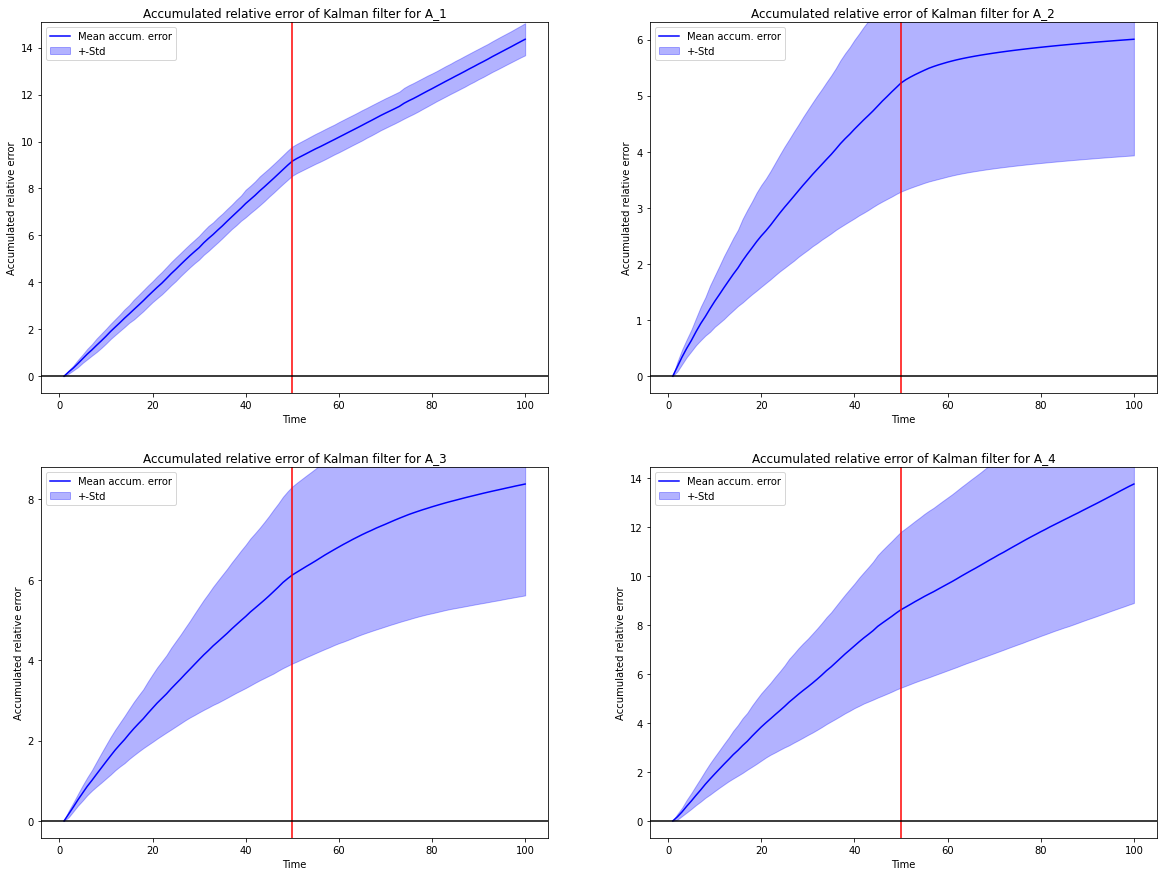
\includegraphics[scale=.6]{figures/kalman_acum}
	\centering
	\caption{Accumulative relative errors' comparative}
\end{figure}

Apreciamos en las gráficas anteriores como a partir de $t=50$ (la línea roja vertical), el crecimiento del error relativo acumulado se reduce considerablmente. Esto es, el error relativo disminuye a partir de dicho instánte. Compararemos los errores de los distintos modelos en detalle en el siguiente apartado. \\

\textbf{Apartado c)} Discutir como los autovalores afectan el error. \\

Para este último apartado haremos uso del error relativo en lugar del error relativo acumulado, será más sencillo visualizar el error en cada instante de esta forma. De forma análoga al apartado anterior, repetimos los experimentos $100$ para cada modelo y computamos la media y desviación típica punto a punto:

\begin{minted}{python}
def plot_errors(models, max_time=100, n_repetitions=100):
	names = [ 'A_{}'.format(i) for i in range(1,5) ]
	x = np.arange(1, max_time+1)
	rel_errors = [
		[ m.simulate_kalman_filter(max_time) for i in range(n_repetitions) ]
		for m in models
	]
	means = np.mean(rel_errors, axis=1)
	stds = np.std(rel_errors, axis=1)
	
	_, axis = plt.subplots(2, 2, figsize=(20,15))  
	axis = np.array(axis).flatten()
	for i in range(4):
		subplot_errors(axis[i], x, means[i], stds[i], names[i])
		axis[i].legend(['Mean error', '+-Std'])

set_seed(123)
plot_errors(models)
\end{minted}

\begin{figure}[H]
	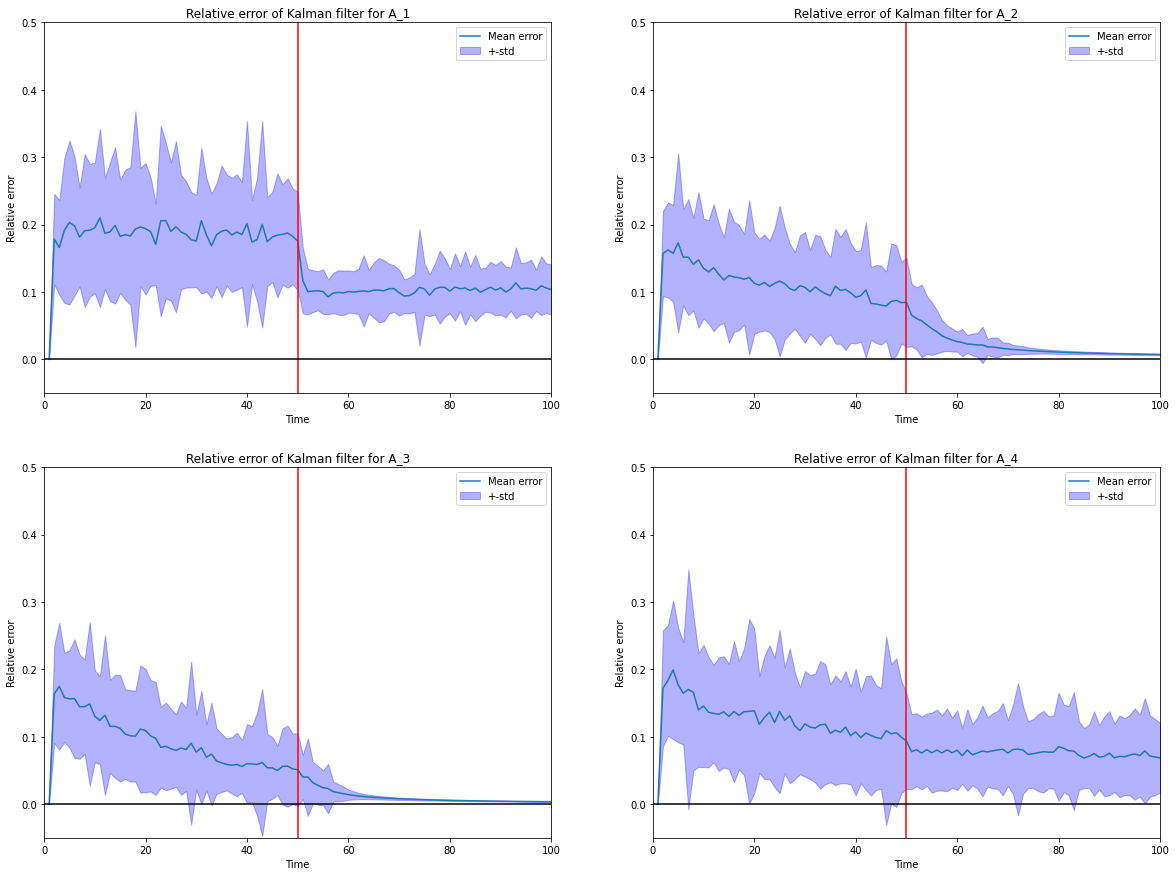
\includegraphics[scale=.6]{figures/kalman1}
	\centering
	\caption{Relative error' comparative}
\end{figure}

Vemos como en este gráfico es notablemente más sencillo comparar los resultados obtenidos. A primera vista resalta como todos los errores pasan a reducirse notablemente a partir de la introducción del input en el instante $t=50$. En particular, los errores de los modelos $2$ y $3$ parecen converger a $0$, siendo la convergencia del segundo modelo ligeramente más rápida. Sin embargo, parece que los errores de los modelos $1$ y $4$ convergen a $0.1$, aunque con oscilaciones. \\

Por otro lado, seguimos observando un alto número de oscilaciones en el error relativo medio a pesar de repetir el experimento $100$ veces. En sucesivos experimentos no presentados en esta memoria se ha observado como la matriz $A$ generada de forma aleatoria estaba introduciendo variabilidad adicional en los resultados del modelo. Es por ello que decimos realizar una experimento adicional para minimizar esta variabilidad. \\

Para ello fijamos un tipo de modelo $i \ in \{1, \ldots, 4\}$, generamos $100$ matrices $A_i$ y para cada una de dichas matrices repetimos el experimento $100$ veces. Presentamos a continuación, para cada modelo, la media punto a punto realizada sobre tanto las $100$ ejecuciones como sobre las distintas $100$ matrices para dicho modelo, en verde. En azul mostramos los resultados del experimento anterior para poder compararlos.

\begin{minted}{python}
def plot_errors_boostrap(max_time=100, n_repetitions=100, n_copies_of_each_model_type=100):
	x = np.arange(1, max_time+1)
	all_models = [
		[ KalmanFilter(get_test_case(i)) for _ in range(n_copies_of_each_model_type) ]
		for i in range(1, 5)
	]
	rel_errors = [
		[
			[ model.simulate_kalman_filter(max_time) for i in range(n_repetitions) ]
			for model in i_models
		]
		for i_models in all_models
	]
	fixed_A_means = [ np.mean(model_A_i_errors[0], axis=0) for model_A_i_errors in rel_errors ]
	fixed_A_stds = [ np.std(model_A_i_errors[0], axis=0) for model_A_i_errors in rel_errors ]
	total_means = np.mean(rel_errors, axis=(1,2))
	total_stds = np.std(rel_errors, axis=(1,2))
	
	names = [ 'A_{}'.format(i) for i in range(1,5) ]
	_, axis = plt.subplots(2, 2, figsize=(20,15))  
	axis = np.array(axis).flatten()
	for i in range(4):
		subplot_errors(axis[i], x, fixed_A_means[i], fixed_A_stds[i], names[i], color='b')
		subplot_errors(axis[i], x, total_means[i], total_stds[i], names[i], color='green')
		axis[i].legend(['A-fixed mean', 'Total mean', 'A-fixed +-Std', 'Total +-Std'])
	
set_seed(123)
plot_errors_boostrap()
\end{minted}

\begin{figure}[H]
	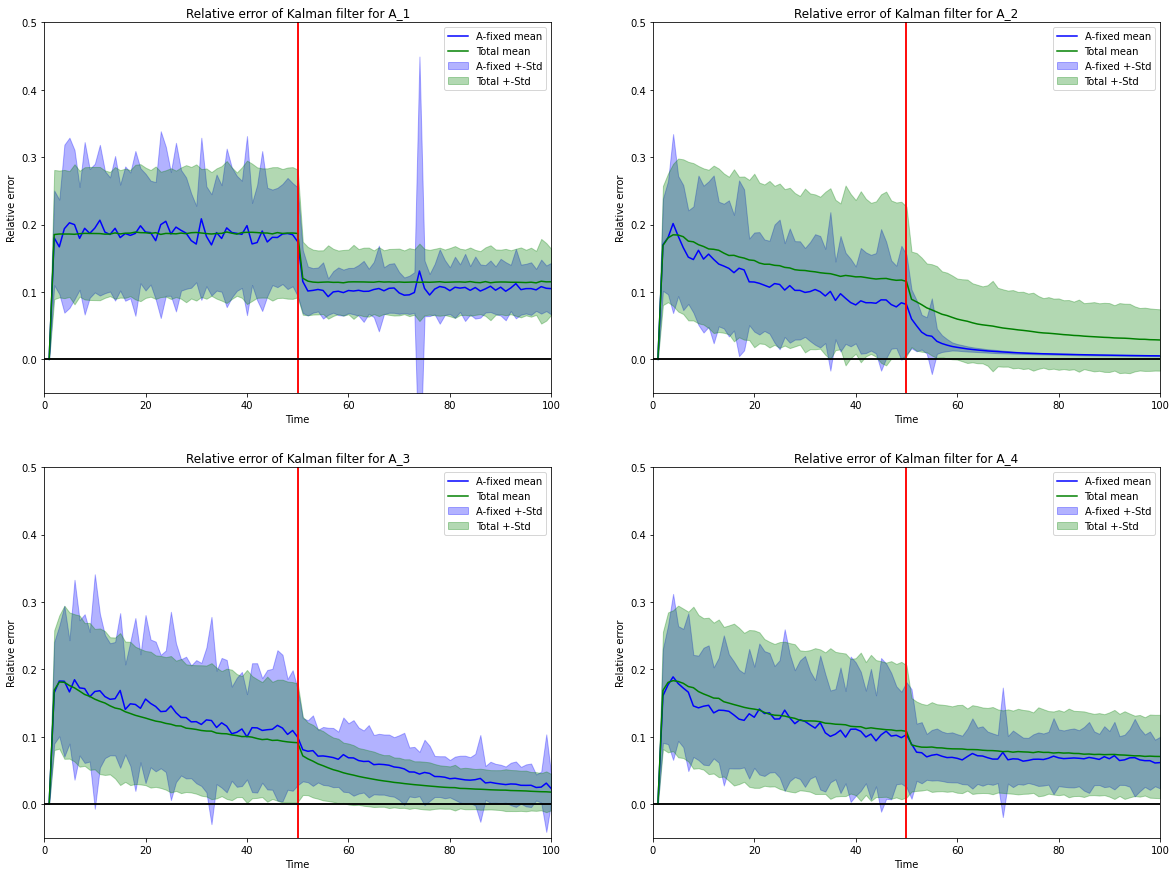
\includegraphics[scale=.6]{figures/kalman2}
	\centering
	\caption{Boostrap relative error' comparative}
\end{figure}

Vemos como efectivamente la variabilidad presente en los resultados anteriores se reduce: tanto el tiempo medio como las desviaciones típicas son más estables y fluctúan más suavamente. Observamos también como en algunos casos el error para el modelo fijado es mayor y en otras ocasiones menor que el error medio sobre múltiples modelos. \\

En particular, apreciamos como nuestra conclusión sobre la rápida convergencia del modelo $2$ fue prematura: si observamos una convergencia a $0$ pero no tan rápida como supusimos. Por otro lado, la convergencia del modelo $3$ es ligeramente más rápida de lo esperado. \\

Finalmente, los modelos $1$ y $4$ siguen pareciendo estabilizarse en $0.1$, aunque observamos una ligera tendencia decreciente en el cuarto. \\

Para estudiar mejor la convergencia de estos sistemas realizamos un experimento adicional, aumentando el tiempo máximo de convergencia a $10^4$ en vez de $100$. Así mismo, reducimos el número de ejecuciones por matriz y de matrices por modelo de $100$ a $20$ (las ejecuciones anteriores ya requerían de unos $10$ minutos). Obtenemos los siguientes resultados:

\begin{minted}{python}
set_seed(123)
plot_errors_boostrap(max_time=10**3, n_repetitions=20, n_copies_of_each_model_type=20)
\end{minted}

\begin{figure}[H]
	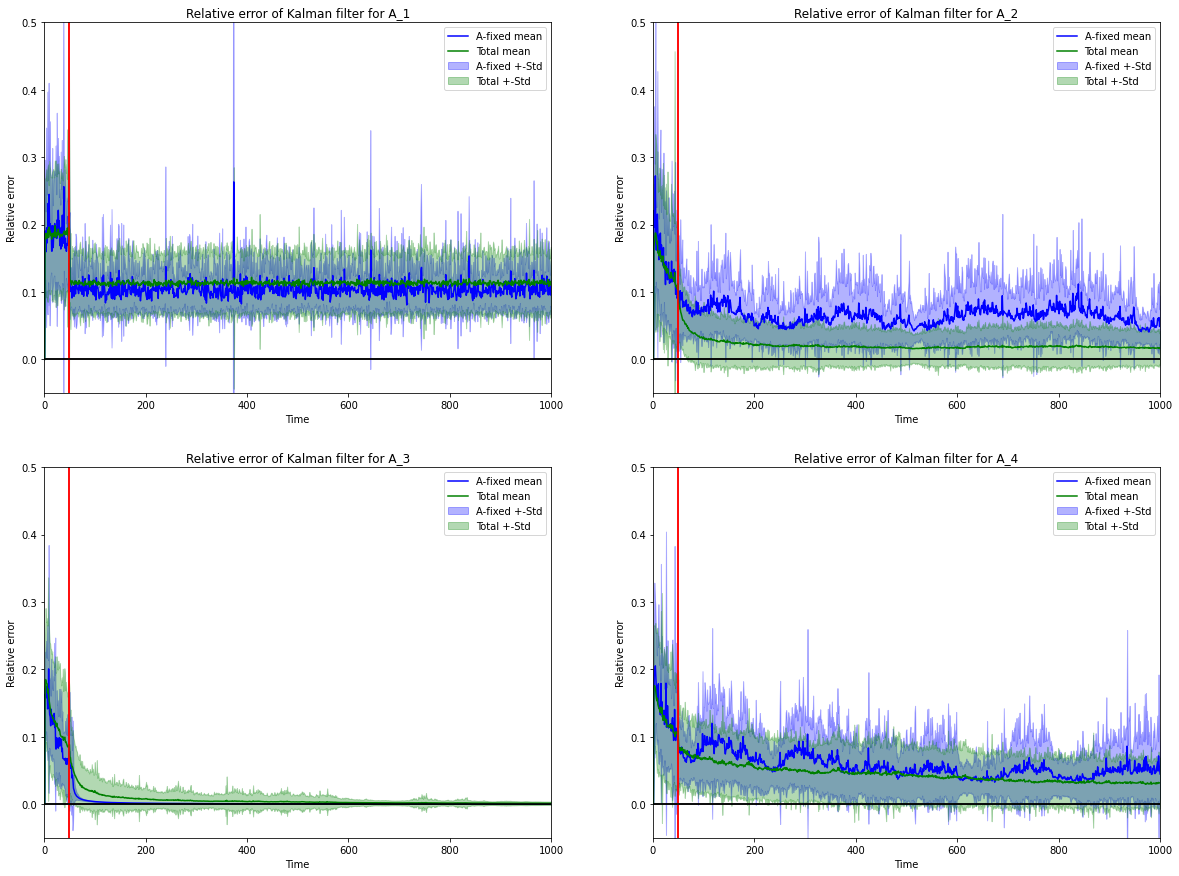
\includegraphics[scale=.6]{figures/kalman3}
	\centering
	\caption{Boostrap relative error' comparative up to $t=10^3$}
\end{figure}

Aunque se ve un aumento sustancial de la variabilidad al disminuir las repeticiones realizadas, podemos sacar buenas conclusiones de resultados:

\begin{enumerate}
	\item El error del primer modelo se estabiliza cercano a $0.11$.
	\item El error del segundo modelo se acerca notablemente más a $0$ pero no parecer estabilizarse sobre $\approx 0.3$. 
	\item El error del tercer modelo converge rápidamente $0$, como ya sospechábamos. 
	\item El error del cuarto modelo parece decrecer muy lentamente. Al llegar a $t=10^3$ se sitúa sobre  $\approx 0.5$, aunque es díficil asegurar mirándo estas gráficas si seguirá decreciendo o se estabilizará. 
\end{enumerate}

Antes de exponer las conclusiones finales, realizamos un experimento adicional para verificar si el cuarto modelo tiene un convergencia muy lenta o si no llega a converger. Para ello aumentamos el tiempo máximo de convergencia a $10^5$ en vez de $10^3$. Así mismo, reducimos el número de ejecuciones por matriz y de matrices por modelo de $20$ a $5$. Esto aumentará notablemente la variabilidad, pero es un mal necesario para realizar ejecucion en tal rango de tiempo.

\begin{minted}{python}
	set_seed(123)
	plot_errors_boostrap(max_time=10**4, n_repetitions=5, n_copies_of_each_model_type=5)
\end{minted}

\begin{figure}[H]
	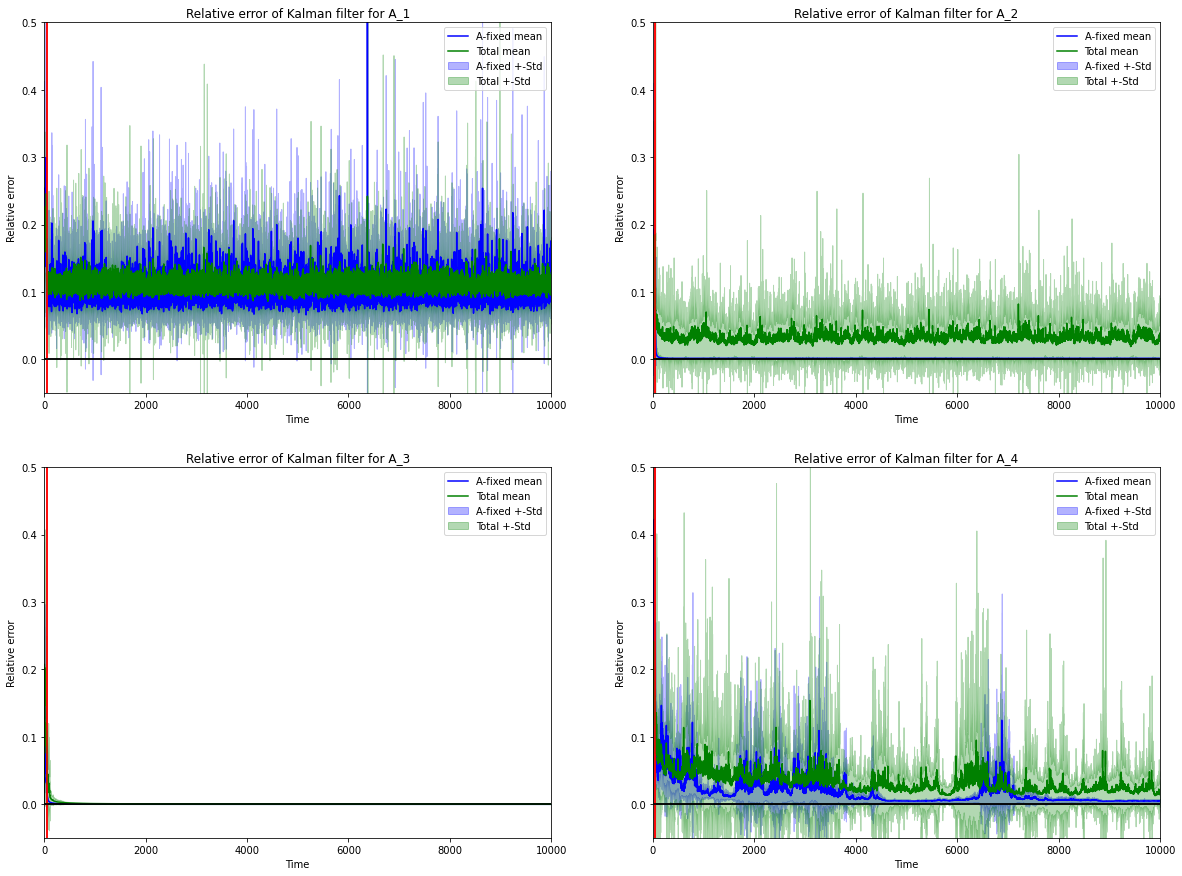
\includegraphics[scale=.6]{figures/kalman4}
	\centering
	\caption{Boostrap relative error' comparative up to $t=10^4$}
\end{figure}

Aunque en la iteración de modelo fijo observamos que hay convergencia a partir de cierto valor, no queda claro observando las medias que este hecho ocurra para todos los modelos posibles. \\

A continuación nos apoyámos en los resultados teóricos de la asignatura para aportar cierta luz sobre el resultado de estos experimentos. En primer lugar, sabemos por el Teorema $5.1$ que todos los valores propios han de estar en $\[-1, 1\]$, y que la multiplicidad del valor propio $1$ no puede ser mayor de $1$. Esto ocurre en todos nuestros modelos. \\

En segundo lugar, sabemos que el valor propio $1$ está asociado a la probabilidad estacionaria $\pi$ (vector propio asociado). Este valor propio está presente en el tercer modelo, es por ello que observamos tal rápida e invariable convergencia. \\

Del mismo modo, observamos que el segundo modelo tiene un valor propio muy cercano a $1$ ($0.99$). Esto se traduce en la casi-convergencia del error a $0$, pues oscilaremos ligeramente sin llegar a converger. \\

Dado que el primer modelo tiene sus valores propios muy lejanos en valor absoluto a $1$, el modelo simplemente oscilará entre sus posibles estados, con probabilidades descritas por la matriz $A$. Esto se traduce en que las predicciones sean bastante improbables.\\

Finalmente, el cuarto modelo presente un valor propio $-1$. Esto significa que el grafo asociado es bipartido. Además, como no tiene ningún valor propio $1$ sabemos que no puede darse convergencia a la probabilidad estacionaria. A pesar de ello, obtenemos errores muy bajos. Mi hipótesis del porqué de este hecho es que al tener un grafo bipartido con unicamente $4$ nodos, nuestra posibilidad de acertar de forma aleatoria es de $1/2$, en vez de $1/4$ como en el caso del primer modelo. \\

Por otro lado, este modelo es ligeramente distinto al planteado en clase. En primer lugar, la matriz $C$ asociada a nuestra medición era $[1,0,0,0]'$, permitiéndonos conocer únicamente el estado anterior. Ahora esta matriz posee dos filas, y nos permite observar dos estados anteriores. \\

Por otro lado y más importante, introducimos un input. No tengo claro como afecta esto a la convergencia en el caso más general, pero en nuestro caso particular, el input será constante a partir de un punto. Esto nos permite nuestro modelo de la siguiente forma, a partir de $t=50$:

\[
	x_{t+1} = A x_t + B u_t + w_t = A x_t + 1 \cdot B + w_t = A x_t + w_t'
	z_t = C x_t + v_t
\]

Donde $\w_t'$ tendrán media $1$ y la misma matriz de covarianzas asociada. Es decir, es un modelo como el que conocemos. Como la varianza del ruido no varía, nuestra predicción será prácticamente igual de acertada. \\

Entonces, ¿por qué vemos una reducción del error relativo a partir del instante $t=50$? La respuesta es sencilla: al sumar uno al sistema completo (tanto a las predicciones como a los valores reales de $x$), el error relativo es más pequeño porque depende de la norma de $x$. Es decir, nuestra predicción es mejor proporcionalmente porque hemos hecho más grandes los números que comparamos, pero la distancia entre ellos es prácticamente equivalente.

\end{document}
